\documentclass[10pt,journal,compsoc]{../IEEE/IEEEtran}

\usepackage[utf8]{inputenc}
\usepackage{todonotes}
\newcommand{\todonaps}[1]{\todo[inline,color=green!40]{#1}}
\newcommand{\todopfac}[1]{\todo[inline,color=red!40]{#1}}
\newcommand{\todoextra}[1]{\todo[inline,color=blue!40]{#1}}
\newcommand{\todorev}[1]{\todo[inline,color=gray!60]{#1}}

\usepackage[colorlinks=true]{hyperref}
\usepackage{cleveref}
\usepackage[cmex10]{amsmath}
\usepackage{algpseudocode}
\usepackage{algorithmicx}
\usepackage{algorithm}
\usepackage{epstopdf}
\usepackage{graphicx}
\usepackage{caption}
\usepackage{subcaption}
% \usepackage{subfig}
% \usepackage[style=ieee, backend=biber, bibencoding=utf8]{biblatex}
% \addbibresource{../bib/strings.bib}
% \addbibresource{../bib/manuals.bib}

% declare the path(s) where your graphic files are
\graphicspath{{images/}}

\usepackage{xspace}
\newcommand{\computeflux}{\texttt{compute\_flux}\xspace}
\newcommand{\update}{\texttt{update}\xspace}
\newcommand{\polu}{\texttt{polu}\xspace}
\newcommand{\dirichlet}{\textit{Dirichlet}\xspace}

\newsavebox{\ieeealgbox}
\newenvironment{alg}
  {
   \begin{lrbox}{\ieeealgbox}
   \begin{minipage}{\dimexpr\columnwidth-2\fboxsep-2\fboxrule}
   \hrulefill
   \begin{algorithmic}
  }
  {
   \end{algorithmic}
   \hrulefill
   \end{minipage}\end{lrbox}\noindent\mbox{\usebox{\ieeealgbox}}
  }

% Add "Appendix" to the appendices titles, but not to the references
\usepackage{ifthen}
\newcommand*{\appendixmore}{%
  \renewcommand*{\othersectionlevelsformat}[1]{%
    \ifthenelse{\equal{##1}{section}}{\appendixname~}{}%
    \csname the##1\endcsname\autodot\enskip}
  \renewcommand*{\sectionmarkformat}{%
    \appendixname~\thesection\autodot\enskip}
}



% correct bad hyphenation here
%\hyphenation{op-tical net-works semi-conduc-tor}

%
% DOCUMENT
%

\begin{document}

%
% TITLE PAGE
%
\title{A Finite Volume Case Study From An Industrial Application}

\author{Miguel~Palhas,~\IEEEmembership{pg19808,~MEI}
        , Pedro~Costa,~\IEEEmembership{pg19830,~MEI}
        and Stéphane~Clain,~\IEEEmembership{co-Advisor}%
  \IEEEcompsocitemizethanks{%
    \IEEEcompsocthanksitem{M. Palhas and P. Costa are with the Department of Informatics at University of Minho, Braga, Portugal\protect\\%
      E-mail: \texttt{pg\{19808,19830\}@alunos.uminho.pt}
    }
    \IEEEcompsocthanksitem{Professor Doctor Stéphane Clain is with the Department of Mathematics and Applications at University of Minho, Braga, Portugal\protect\\%
      E-mail: \texttt{clain@math.uminho.pt}
    }
  }
}

\markboth{Integrated Project, Parallel and Distributed Computing, June~2012}%
{Palhas and Costa: A Finite Volume Case Study From An Industrial Application}


% use for special paper notices
%\IEEEspecialpapernotice{(Invited Paper)}


%
% ABSTRACT
%
% for Computer Society papers, we must declare the abstract and index terms
% PRIOR to the title within the \IEEEcompsoctitleabstractindextext IEEEtran
% command as these need to go into the title area created by \maketitle.
\IEEEcompsoctitleabstractindextext{%
\begin{abstract}
%\boldmath
\todo[inline]{This template is quite acceptable for a paper, but IMO it is unfit for a technical/scientific report for a class. SCREW YOU. A tua prima!}


\end{abstract}
% IEEEtran.cls defaults to using nonbold math in the Abstract.
% This preserves the distinction between vectors and scalars. However,
% if the journal you are submitting to favors bold math in the abstract,
% then you can use LaTeX's standard command \boldmath at the very start
% of the abstract to achieve this. Many IEEE journals frown on math
% in the abstract anyway. In particular, the Computer Society does
% not want either math or citations to appear in the abstract.

% Note that keywords are not normally used for peerreview papers.
\begin{IEEEkeywords}
Integrated Project, Finite Volume, mesh, C/C++, OpenMP, MPI, CUDA
\end{IEEEkeywords}
}


% make the title area
\maketitle

%
% BODY
%

\section{Introduction}
\label{sec:intro}

This document describes an incremental work where the \texttt{polu} application, which computes the propagation of a pollutant in a two dimensional environment, was studied in order to find possibilities of optimization and/or parallelization.

The \texttt{polu} application is built on top of the Finite Volume Library (FVL) which is also a focus of study in this document, as a large part of the logic and data structures are implemented on it, rather than on the application itself. In this context, both of them are considered as a whole case study.

Several changes were performed in the original code, which are fully described in this document. Those changes vary in nature, from simple or low-level code optimization, to higher-level algorithmic changes, in order to allow parallelization and/or improve performance. The data structures used also suffered large changes (originally implemented as \textit{Arrays-of-Pointers}) to \textit{Arrays-of-Structures} at first, and also to \textit{Structure-of-Arrays}. This changes removed excessive dereferencing caused by deep chains of pointers in the original strucutres, effectively reducing memory accesses and improving locality.

The several phases that composed this project reflect on the multiple approaches and variety of results presented here. In general, the goal is to study the performance impact, advantages and difficulties of different programming paradigms, applied to the \texttt{polu} application. 


\todo[inline]{O paragrafo aqui a explicar o que é falado no relatorio}

After the initial analysis of initial sequential code, a shared-memory parallel implementation, using OpenMP \todo{ref sec:omp}, a distributed-memory implementation, with the \textit{Message Passing Interface} (MPI) \todo{ref sec:mpi}, and a GPU implementation (using CUDA) \todo{ref sec:cuda} were implemented and profiled.

\section{Case Study}
\todo[inline]{Explain what the program is meant for}

The application analyzed in this document computes, called here \texttt{polu}, computes the flux of a material (e.g. a pollutant) through a bidimensional surface. This surface is described as a mesh, composed mainly of edges and cells. The input is given by a 

The original \texttt{polu} application works like a heartbeat algorithm with no communication (since it is executed in a single computation node). The algorithm used by the application sees the environment as a discrete mesh (represented by its cells and edges) and loops until the specified time interval is reached. At each iteration of this main loop, the algorithm performs two main steps:

\begin{description}[\IEEEsetlabelwidth{Pollution Update}\IEEEusemathlabelsep]
	\item[Flux Computation] Based on current pollution values for each cell, the flux for each edge is calculated (performed by the \texttt{compute\_flux} function)
	\item[Pollution Update] Using the previously calculated flux values, the pollution for each cell is updated (performed by the \texttt{update} function)
\end{description}

\subsection{Algorithm}

The algorithm used by the \polu application is a first order finite volume method. This means that each mesh element only communicates directly with its first level neighbors in the mesh, which makes this a typical case of a stencil computation. In terms of performance, being a stencil algorithm implies that the operational intensity \todo[inline]{ref ao paper do roofline} will most likely remain constant with larger problem sizes. On the other hand, the low order allows for a greater locality of the calculations, and favors parallelization.

The code consists on a preparation stage, where all the required elements are loaded and prepared, and two computation stages, which compose the main loop.

Operations performed in the preparation stage are highly dependent on the implementation being described, as most will require some elements to be properly organized or some values to be previously computed. Common operations, such as loading the necessary data from the described files are constant to every implementation, but may still differ in the structures used to store the data.

A single execution of the two computation stages together form a step in the iterative method behind this application. These stages, also referred in this document as core functions, or kernels, are the \computeflux and \update functions.

In \computeflux, all the edges in the mesh are analyzed, and the flux of pollution to be transfered across that edge is computed, based on the polution level and the velocity vectors of the cells it connects. A preconfigured value is used as the \dirichlet condition\footnote{The \dirichlet condition is a type of boundary condition used to specify a value taken by the solution in the border of the domain. In the \polu application, this value is constant throughout the execution}, which replaces the polution level of a second cell for the edges in the border of the mesh.

As for the \update function, it uses the computed flux values to update the polution levels of each cell in the mesh, by adding the individual contribution of each edge of the cell. While triangular cells are prefered, there are no restrictions to the number of edges a cell may have.

\subsection{Parallelism Oportunities}
\todo[inline]{Explain what can be executed in parallel}
\todo[inline]{Mention this is a heartbeat}

During the main loop of this program both core functions, \computeflux and \update, depend on each other to perform their tasks. \update requires flux from all edges to be previously computed in \computeflux, which in turn requires that all pollution values are up-to-date to correctly compute the flux for the next iteration. This creates two implicit synchronization points in the main loop, and is a consequence of the heartbeat characteristics of the problem.

This allows both functions to be looked at as individual tasks, that may be subject to different parallelization approaches. Both functions perform calculations using the entire mesh, but they differ in the element used: while \computeflux iterates over edges, \update iterates over cells.

\todo[inline,color=green!40]{Ainda tentei acabar eu isto mas não sei bem onde querias ir com este texto, por isso acaba tu. Pode ser útil um parágrafo a explicar que nos algoritmos de stencil é comum deixar-se que diferentes partes da mesh estejam em diferentes iterações por só terem dependência local, mas que no nosso caso por ser um heartbeat isto não é de todo trivial de implementar.}

\section{Sequential}
\label{sec:seq}

\todorev{Written on Sat, June 30 at 13:16 by pfac}

In this section are presented the sequential implementations of \polu, from the original to the optimized versions. \Cref{sec:seq:limitations} analyzes the dependencies in the sequential code which prevent the parallelization of the core functions (as explained in \cref{sec:220}), and how the code was adapted to remove them. 

\subsection{Original}
\label{sec:310}
%\todo[inline,color=blue!40]{Add some algebra to the core functions text. Hard to keep track with only text.}

The original \polu program was implemented using structures as \textit{Arrays-Of-Pointers} (AOP). While this allows for an easier development and better code readability, the deep levels of dereferencing imply an increased number of memory accesses, which aggravate the effects of any memory bottlenecks.

In this original version, the \computeflux function iterates over each edge, and loads the pollution levels and velocity vectors of the cells it connects. For edges in the border of the mesh, a convention is followed, indicating that the non existing cell is alwasy the right one (cells are refered to as left and right cells of a given edge). When the right cell doesn't exist, the \dirichlet condition is used as the value for that border.

The velocity vector in the edge is computed based on the velocity of both cells and the normal of the edge. This final velocity also gives information about the direction of the flux. A positive velocity makes the pollution flow from left to right, and the inverse happens with a negative velocity. \Cref{alg:flux} illustrates this behavious.



\begin{figure}[!htp]
	\begin{alg}
		\ForAll {$edge \in Edges$}				\\
			$l     \gets left\_cells_{edge}$ 	\\
			$r     \gets rigth\_cells_{edge}$ 	\\
			$u_{l} \gets pollution_{l}$ 		
			\If {$\exists Cells_{r}$} 			\\
				$u_{r} \gets pollution_{r}$
			\Else 								\\
				$u_{r} \gets \dirichlet$ 
			\EndIf 	 							\\
			$v_{edge} \gets (v_{l} + v_{r}) / 2 \cdot normal_{edge}$ 					\\
			$v_{max} \gets max(v_{max}, v_{edge})$ 										\\
			$flux_{edge} += u_{l} \cdot [v_{edge}]^{+} + u_{r} \cdot [v_{edge}]^{-}$
		\EndFor
	\end{alg}

	\caption{Pseudocode for the original \computeflux function}
	\label{alg:flux}
\end{figure}

This function also returns the elapsed time, which is computed with the maximum absolute value of the computed edge velocities, and is used at the end of the iteration to keep track of the total elapsed time.

The original \update function also iterates over each edge. The contribution of each edge to the cells final value is computed as the product between the elapsed time, the computed flux and the ratio between the edge's length and the cell's area. This is described in \cref{alg:update}.

\begin{figure}[!htp]
	\begin{alg}
		\ForAll {$edge \in Edges$}

			$\Delta{u} \gets \Delta{t} \cdot flux_{edge} \cdot L_{edge}$

			$l \gets left\_cells_{edge}$

			$r \gets right\_cells_{edge}$

			$pollution_{l} -= \frac{\Delta{u}}{A_{l}}$

			\If {$\exists Cells_{r}$}

				$pollution_{r} \gets \frac{\Delta{u}}{A_{r}}$
			\EndIf
		\EndFor
	\end{alg}

	\caption{Original \update function}
	\label{alg:update}
\end{figure}



There is also the possibility to output the current state of the mesh after every $X$ of iterations, where $X$ is a parameter provided at runtime. This feature allows the output to contain not only the final state of the system byt all the intermediary states, allowing  an animation to be shown using \texttt{gmsh}.

\subsubsection{Simplifications}
% \todo[inline]{Animation and velocity calculation are out}

Two important simplifications were initially performed in the original version, before any other adaptation or rewrite of the code.

The first simplification meant removing the output operation at the end of each main loop iteration, thus removing the animation feature. While this feature is interesting to analyze how the system evolved, input/output operations are very slow when compared to computation operations. Since the main goal of this document is to study ways to improve the performance of the \polu application, this feature may be discarded.

The second major simplification focus on the \computeflux function. Since the every cell's velocity vector remains constant throughout the entire program's execution, the same values will be computed for the velocity in each edge and for the elapsed time. While this computation is important in a more dynamic application where velocity vectors are also updated, such is not the case for this algorithm. Therefore, it is possible to remove these two computational steps from the core function to the preprocessing stage, thus globally improving the program's performance.

\subsection{Optimizations}
\label{sec:seq:optimizations}

\todorev{Last revised on Sat, June 30 at 15:33 by pfac}

While optimizing the sequential code may be important to eliminate possible bottlenecks created by inefficient memory access patterns or poorly written code, most of the optimization work was kept for after the parallelization, as early optimizations might have hampered parallel implementations.
As such, the focus of optimization in the sequential implementation of \polu was on the structures used, which were trivially found to be very inefficient.

As previously stated, the original implementation relied on an AOP approach, but the excessively deep chains of pointers translate into more memory accesses, and consecutively worse performance.

The next two sections describe the two alternative approaches and explain how these improved the application's performance.

\subsubsection{AOS}
% \todo[inline]{Explain the AOS structures and why they should be better than AOP}

The first implemented alternative to AOP was the \textit{Arrays-Of-Structs} approach. Instead of using pointers, structures were created for cells and edges, containing all the data about each. Where pointers existed to link an edge to the adjacent cells, or a cell to its edges, an index is placed. While the dereferencing levels are completely eliminated, using indexes allows any element to hold identifiers which allows direct access to the other elements it needs to interact with, as long as all the data objects are stored in arrays. The maximum representable index is used as the equivalent to \texttt{NULL} pointers (applied, for example, to the right cell of a border edge).
\subsubsection{SOA}
% \todo[inline]{Explain the SOA structures and why they should be better than SOA}

While the AOS approach completely removes the need for dereference, using a \textit{Struct-Of-Arrays} (SOA) approach can be more efficient.

One of the problems with the AOS approach is that when the core functions iterate over one of the arrays, cache lines are being filled with the complete structure of these elements. Yet, neither of the core functions utilizes all the data in that structure, which translates in useless data occupying the cache. This hurts spatial locality\footnote{If a data element is required, it is highly probable adjacent elements will also be required in the near future.}, greatly increasing the chances of accessing a mesh element translating into a RAM access.

The SOA approach solves this problem by placing the data of each element in distinct. As an example, a single array is created to hold the polution level of all the cells. Each data piece is placed in a different array.

This approach allows the core functions to load only the data required for their compuations. The cache lines are now filled only with useful data, and the pieces which are required by the other functions will only be loaded when needed.
\subsubsection{Results}

\todorev{Written on Sat, June 30 at 21:40 by pfac}

To evaluate the impact of the optimizations presented in \cref{sec:321,sec:322}, performance tests were performed with the original and optimized versions.
\Cref{sec:env,sec:method} describe the environmental setup and methodology for the tests performed, respectively.

\Cref{fig:seq:results} shows the results obtained for the three sequential versions.
Both optimized versions show a clear improvement just by not using the several dereference levels. Also, the results show a clear improvement by using SOA over AOS, proving the effectiveness of the optimization.

\begin{figure}[!htp]
	\centering
	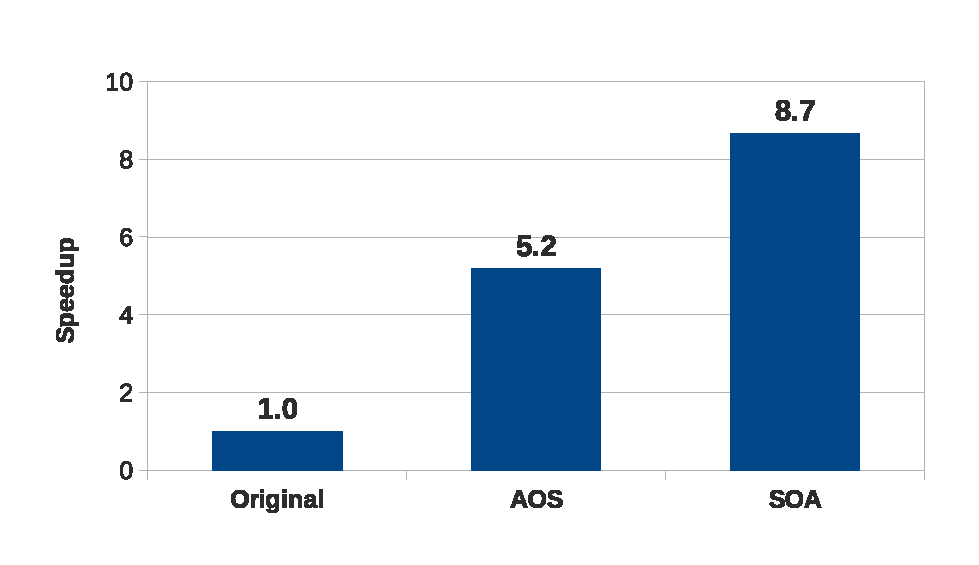
\includegraphics[width=\columnwidth]{images/graph_comparison_seq.eps}
	\caption{Speedup results for the three sequential versions, compared with the original version.}
	\label{fig:seq:results}
\end{figure}
\subsection{Limitations}

The main limitation for the sequential versions is the locality of the mesh used in the problem. Since this issue will be present in any shared memory implementation too, that discussion is left for \cref{sec:omp:limitations}.

\Cref{fig:roofline} shows the roofine for SeARCH Group 201 with the computational intensities of the SOA and AOS versions. Computational intensity is defined to be the ratio between all the instructions not related with memory accesses (loads and stores) and the number of bytes accessed in RAM.

The improvement from AOS to SOA can be explained only by the improvements in locality. Further testing, which results were omitted in this document, shown that the number of bytes acessed to RAM, number of computational instructions completed and the core functions execution time all decreased, achieving almost the same amount of computational instructions per second, while halving the number of accesses.

\begin{figure}
	\centering
	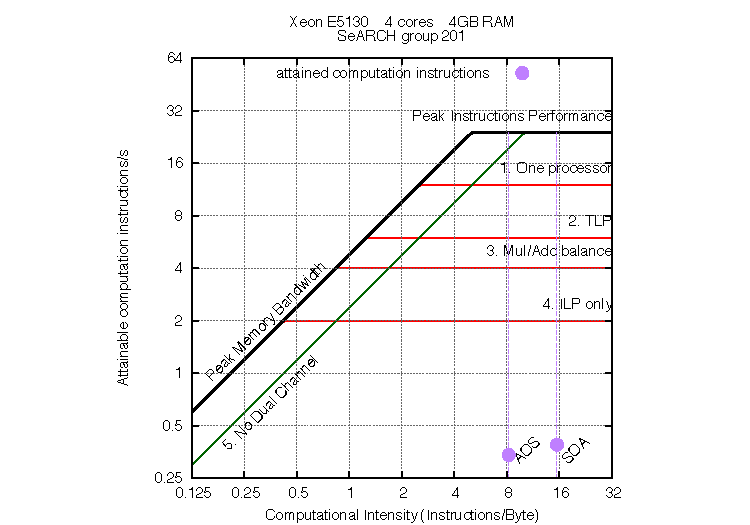
\includegraphics[width=\columnwidth]{images/roofline201m.pdf}
	\caption{Roofline for SeARCH Group 201, with the computational intensities of the AOS and SOA versions.}
	\label{fig:roofline201}
\end{figure}

\subsection{Dependencies}
\label{sec:dependencies}

\todorev{Last revised on Sat, June 30 at 21:47 by pfac}

\todoextra{Maybe add here a footnote to explain reductions.} 

As explained in \cref{sec:220}, the heartbeat nature of the algorithm prevents extending parallelization beyond the scope of each core function, but both functions are able to execute their internal iterations in parallel.
Yet, some dependencies exist among the elements used in these functions, and adaptations are required to allow parallelization.

\computeflux has only one dependency, in the computation of the elapsed time $\Delta t$, which is removed simply by accepting the second simplification described in \cref{sec:311}.
While this simplification is assumed in the final implementations, this dependency was properly studied in early stages of the project.
Since the computation of $\Delta t$ is based in a maximum operation, it is possible to replace this dependency with a reduction after the computation of the fluxes, thus removing the dependency and maintaining the correctness of the program.

On the other hand, the \update function has a dependency which may not be neglected because of a simplification.
As described in \cref{sec:310}, the original implementation of \update iterates over the edges.
While this may favor locality after executing \computeflux, it creates a race condition when each edges adds its own contribution to the cell's value.
This dependency can be removed by changing how \update iterates over the mesh. By iterating over the cells instead of the edges, the race condition disappears since only one write operation per cell is performed, as shown in \cref{alg:update}.

\begin{figure}[!htp]
	\begin{alg}
		\ForAll {$cell \in Cells$}
			\ForAll {$edge \in Edges_{cell}$}
				\State $pollution_{cell} += \Delta{t} \times flux_{edge} \times \frac{L_{edge}}{A_{cell}}$
			\EndFor
		\EndFor
	\end{alg}

	\caption{New \update function, now iterating over cells instead of edges}
	\label{alg:update2}
\end{figure}

\section{Shared Memory}

A shared memory parallel version of \polu was implemented using the OpenMP interface. The main feature about this API is that the program itself remains almost equal to the sequential version, requiring only the addition of the necessary directives and the adaptation of the code to remove dependencies.

Both core functions were parallelized adding a \texttt{parallel for} directive to the internal loops. The number of threads issued in each parallel zone is given as the second argument of the program, and defaults to the maximum number of threads supported by the hardware in the absence of the argument.

	\subsection{Load Balance}
% \todo[inline]{Describe the static scheduling with OpenMP and explain that all the iterations make the same operations in every function}

Both core functions are mostly homogeneous in its parallel implementation. In \computeflux, the two branches perform the same amount of operations whether they are followed or not. In \update, the heaviest part of the workload is constant (products and divisions), and it only differs in the number of edges contributing to the edge. While this value may cause the function to become heterogeneous, this is highly dependent on the mesh used (the test case used in \cref{sec:700} has 3 edges in every cell).

By default, the OpenMP interface uses static scheduling, where iterations are assigned to threads in a \textit{round-robin} pattern. Since the number of edges and cells is a constant throughout the entire execution, this guarantees the best load balancing among threads.

\subsection{Limitations}
% \todo[inline]{Describe the locality problems}
% \todo[inline]{Opportunity to show here that cute image that displays locality of the mesh}

The main problem with this implemetation is data locality. While these issues are softened using a SOA approach, and the method is a first order one, the algorithm is still not very cache friendly in either of the core functions.

In \computeflux, each edge requires access to data from the two adjacent cells. While the access to edges is contiguous, access to cells is not for most of the iterations. Yet, border edges do not require the second edge.

\update on the other hand requires access to all the edges in a cell, which are always more than two. Analogously, the access to cells is contiguous, but the access to edges is not. Since each edge has more edges, than an edge has adjacent cells, and since no edge may be neglect for any cell, this function is most likely the bottleneck of the main loop.
\section{Distributed Memory}
\label{sec:mpi}

For a distributed memory implementation, The \textit{Message Passing Interface} (MPI) was used. With the sequential code having already suffered some changes and optimizations, the main problem consisted in the partitioning of the mesh. The obvious approach is one where each processor is assigned to a subset of the entire mesh, and is responsible for the application of both kernels to its subset. Communication is also required between each main loop iteration, since each process will require access to the values in the border of its subset, in order to compute its own values.

\subsection{Mesh Partitioning}
\label{subsec:mpi:partitioning}

In order to distribute processing payload across each process, the input mesh, and all of the data associated with it, also needs to be split into partitions. A mesh partitioning algorithm is required. This algorithm must generate $P$ disjoined partitions (where $P$ is the number of processors available), each to be assigned to a different processor. Some additional data is also required for each partition, so that information about how each partition connects to the others is kept, to allow communication to be done correctly.

\subsubsection{Research in Mesh Partitioning}
\label{subsubsec:mpi:partitioning:research}

Mesh partitioning is currently an actively researched topic, with some projects and libraries begin already available that help with the understanding of how a mesh (or more generically, a graph) can be partitioned in ways to optimize certain aspects like load balancing, communication balancing or partitioning overhead. For instance, in \cite{metis}, a library called \texttt{Metis} is presented whose purpose is precisely this problem. Other works found for this topic included \cite{gilbert1995, walshaw2000}.

However, given the time constraints of this project, and since the priority was to have a functional algorithm rather than an optimal one, it was decided not to attempt an approach involving \texttt{Metis} or any other researched work. Actually, the method used to partition the mesh is quite naive, as shown in \cref{subsubsec:mpi:partitioning:method}.

\subsubsection{Partitioning Methodology}
\label{subsubsec:mpi:partitioning:method}

he algorithm created to partition the mesh works by dividing it in slices by the horizontal coordinate of each cell. Givem a mesh with a total of 100 cells, and a pool of $P$ processes, the mesh is divided into $P$ partitions, each with exactly $N=100/P$ cells, differing by at most one cell when they cannot be evenly divided. By ordering the cells based on their $x$ coordinate, they are sequentially assigned to each process, in such a way that the first process receives the first $N$ cells of the set, and so on.

\begin{figure}[!htp]
	\begin{subfigure}[b]{0.5\columnwidth}
		\centering
		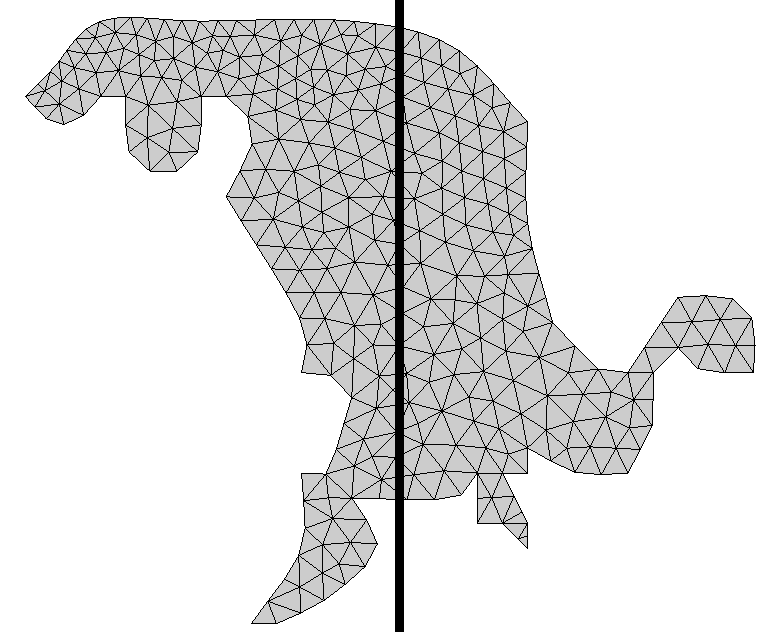
\includegraphics[width=\columnwidth]{foz_p2_msh}
		\caption{2 partitions}
		\label{fig:foz_p2_msh}
	\end{subfigure}%
	\begin{subfigure}[b]{0.5\columnwidth}
		\centering
		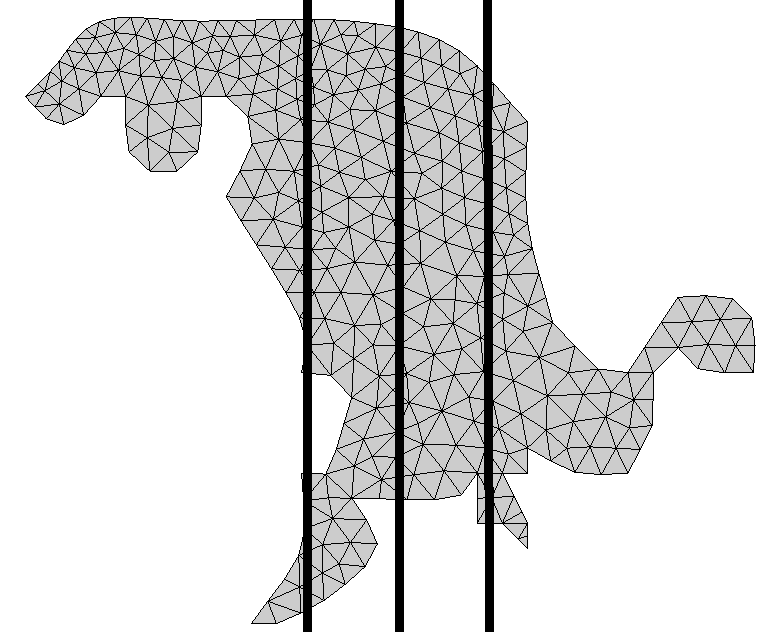
\includegraphics[width=\columnwidth]{foz_p4_msh}
		\caption{4 partitions}
		\label{fig:foz_p4_msh}
	\end{subfigure}%

	\caption{Mesh partitioning illustration}
	\label{fig:partitioning}
\end{figure}

With this partitioning method, communication is also greatly simplified, as it is guaranteed that every partition will have a left and a right neighbor. It is also assumed that the width of the global mesh is big enough so that there are never processes with 0 cells assigned, which would break communication. Since a common mesh usually contains at least thousands of cells, this should not be an issue.
On the other hand, the partitioning and assignement of the cells is done sequentially, and will increase preparation time.

\subsection{Communication Analysis}
\label{subsec:mpi:comm}

When computing the flux for a given edge, the pollution values of both adjacent cells are required. Until now, only one divergent case existed, when the edge was in the border of the mesh. With the addition of partitioning, a new divergence is created, when the edge is not in the border of the global mesh, but in the border of the local partition, meaning that one of its adjacent cells was assigned to a different partition.

A communication step is required at this point, so that each edge in the local border (the border that connects to another partition, not the global mesh border) receives the corresponding values from the neighbor partition 

This communication step was introduced at the beginning of the main loop, and consists of two smaller steps, one for left communication, and one for right communication.
Each iteration, every process starts by communicating the left border values, which were previously indexed in the preparation stage, to its left neighbor. Asynchronously with that task, it receives an equivalent message from the right neighbor, which is also at the same step. After both tasks, the direction of communication is reversed, and the right border values are sent to the right neighbor of each partition.

Only after all communication is done for this process can it continue to the main kernels of the loop. This introduces a large overhead, as it will most likely require a network transfer if the neighbor partition is located in a different machine. This overhead may become a huge bottleneck for the loop, especially for smaller inputs, where the time spent in the kernels is small enough to make the partitioning and communication occupy a large percentage of the program.

An alternative could consist in making the communication an asynchronous task, allowing the flux for inner edges to be computed while the communication is taking place, since they don't depend on the values to be received. Again, due to time constraints, it was not possible to better analyse this solution.

\subsection{Load Balance}
\label{subsec:mpi:load}

\todorev{Last revised on Sat, June 30 at 23:15 by pfac}

With the naive partitioning strategy used, load balance becomes a problem.
The computation itself is actually well balanced, since it is assured that every partition has the same amount of cells (differing at most by one). The problem is in the border between those partitions.
With the division by the horizontal coordinate being used, it becomes obvious that the size of the border between partitions becomes extremely dependant on the format of the mesh itself.
Other approaches, already mentioned in \cref{subsubsec:mpi:partitioning:research} attempt to deal with this, and produce partitions that minimize the size of the border.

The drawback of not controlling border sizes comes at the communication step.
Not only a different partitioning solution could minimize the border, thus minimizing the amount of data transfered, it can also happen that different partitions have very different border sizes, compromising communication balance.

\todonaps{Anhe? Esta última frase faz grande sentido para mim.}


\section{CUDA Implementation}
\label{sec:600}

\todosec{CUDA implementation}
Part of the work of this project was to study the parallelization methods and issues of finite volume schemes in a massively parallel architecture, specifically a GPU, using CUDA as the development technology. Some considerations can be made about the parallelization of each of the schemes presented.

The first-order scheme is the simpler one, with each value of the solution at the end of each iteration being computed based only on the strictly adjacent elements of the mesh. As a result, it should come as no surprise that it was also the one that showed better performance. The higher locality gained from only using adjacent values for each edge allows for much greater locality and less memory overhead than the second-order counterparts.

As for the second-order schemes, before any actual measurements were done, it was expected that the MUSCL would provide a greater occupancy of the GPU, which does not necessarily mean its execution time would be better. The MOOD method spends a significant portion of its time fixing errors on the detected cells. Since these cells usually represent a very small percentage of the entire domain, this means that most of the computational units will be idle, or doing useless work. In MUSCL, this is not the case, as for every interface there is a strict process of building the initial reconstruction, computing the $\Phi$ limiter for that interface, and then limit the reconstruction.
\section{Final results}
\subsection{Results}
\todo[inline]{Only describe the results, a.k.a. translate every chart to words}
\subsection{Analysis}
\todo[inline]{Interpret every chart. Say what each means, what can be concluded from it}
\todo[inline]{Merge this subsection with the results if time is of the essence}
\section{Conclusion}
\label{sec:conclusion}

\todo[inline]{Sum all this shit up.}
\todo[inline,color=green!40]{Or in my own words: Sum the fuck out of this shit}
\todopfac{Mencionar localidade como trabalho futuro.}
\todo[inline]{Referir que apesar dos speedups de CUDA não serem tão melhores que os outros como se esperava, isso pode dever-se ao facto de que não nos foi possivel gerar um input grande o suficiente para tirar o maximo partido do hardware do GPU}

In this report, the analysis of the \polu application and the successive attempts to optimize and parallelize it were presented.

The original implementation presented several performance problems, the most troubling being the structures implemented as \aop. It also presented features which were not fully implemented or not targeted for improving the results of the computation. These features were removed. The main optimizations performed in the sequential implementation involved changing how the structutes were implemented to \aos, and then to \soa, which achieved the best results (almost 10 times faster).
Dependencies existed in the original code, which were removed along with the discarded features and some code adaptations.

Several approaches to parallelism were described. The first implementation, shared memory, used the OpenMP interface to parallelize the two core functions. It achieved a nearly perfect load balance but remained, just like the sequential version, highly limited by the lack of locality in the mesh structure. The \soa version also achieved the best results with this implementation



%
% BIBLIOGRAPHY
%
\bibliographystyle{IEEEtran}
\bibliography{../bib/strings,../bib/articles,../bib/inproceedings,../bib/manuals,../bib/misc,../bib/techreports}

% \printbibliography

%
% APPENDIXES
%

\appendices
\section{Environmental Setup}
\label[appendix]{sec:env}

\todorev{Written on Sun, July 1 at 17:33 by pfac}

The tests described in this document were performed using a very specific subset of nodes from the SeARCH\footnote{\url{http://search.di.uminho.pt}}, here referred as SeARCH Group Hex.

Nodes in SeARCH Group Hex have two hex-core processors (with \intel HyperThreading technology) and 12 to 48 GB of RAM.Further detail regarding the hardware of these nodes can be found in \cref{tab:grouphex}.

These nodes were used for every test performed in this document.
Sequential, shared memory and GPU tests relied used only one node, where tests for distributed memory used two distinct nodes. Inside this group, tests were only limited to the subset with the highest processor clock frequency, not making any distiction between the nodes.
The only exceptions are the GPU tests which used a very specific node with a Tesla M2070 GPU computing module.
Further detail regarding this GPU module can be found in \cref{tab:m2070}.

\begin{table}[!htp]
	\begin{center}
		\begin{tabular}{lc}
			\hline
			Processors per node: & 2	\\
			Processor model: & \intel\xeon X5650\\
			Cores per processor: & 6	\\
			Threads per core: & 2	\\
			Clock frequency: & 2.66 GHz	\\
			\hline
			L1 cache: & 32 KB + 32 KB per core	\\
			L2 cache: & 256 KB per core	\\
			L3 cache: & 12 MB shared	\\
			RAM: & 12 to 48 GB	\\
			\hline
		\end{tabular}
		\caption[SeARCH Group Hex hardware description]{SeARCH Group Hex hardware description. See \cite{xeon5600} for further detail about this processor.}
		\label{tab:grouphex}
	\end{center}
\end{table}

\begin{table}[!htp]
	\begin{center}
		\begin{tabular}{lc}
			\hline
			GPUs per node: & 1	\\
			Model: & \tesla M2070\\
			CUDA cores: & 448	\\
			Peak (double): & 515 Gflops	\\
			\hline
			Dedicated Memory: & 6 GB	\\
			Bandwidth: & 148 GB/s\\
			\hline
		\end{tabular}
		\caption[SeARCH Group Hex GPU computing module hardware description]{SeARCH Group Hex GPU computing module hardware description. See \cite{teslaM2070} for further detail about this processor.}
		\label{tab:grouphex}
	\end{center}
\end{table}

Results obtained in a second type of nodes are shown in this document only to present a roofline.
While this roofline should refer to the SeARCH Group Hex, this being the environment used for comparison, in previous stage of this project the \texttt{PAPI} library could only be used in a very specific node of SeARCH Group 201.
Build the roofline for the Group Hex nodes, which meant rerunning tests with the \texttt{PAPI} library, was not possible in this stage due to time constrictions.
Attempts were made in previous project stages, but the STREAM benchmark\footnote{\url{http://www.cs.virginia.edu/stream/}} returned less memory bandwidth than in Group 201, which is not true.
Later analysis showed the problem was in the fact that such benchmark must not be run in Group Hex nodes using all the supported parallelism (6 threads, instead of 24, achieved around 15 GB/s).
\section{Experiment Methodology}
\label{sec:method}

\todo[inline]{Explain the hows and whys of the latest methodology}
\todo[inline]{Add the methodologies from all the phases which were not retested}
\todo[inline]{No problem in sending this to an appendix -> and it should}




\end{document}


